\documentclass[sigconf,anonymous]{acmart}
% Submission draft. Numbers come from research/paper_draft.md (the lab log); run directories are
% listed in Appendix F, not in the text.

\settopmatter{printacmref=false, printccs=false, printfolios=true}
\setcopyright{none}
\renewcommand\footnotetextcopyrightpermission[1]{}
\acmConference[Preprint]{Under review}{2026}{}
\acmYear{2026}

\usepackage{booktabs}
\usepackage{multirow}
\usepackage{algorithm}
\usepackage{algpseudocode}
\usepackage{tikz}
\usetikzlibrary{arrows.meta,positioning,fit,calc,backgrounds}
\graphicspath{{figures/}}
\emergencystretch=1em

\newcommand{\lp}{\ell}
\newcommand{\nl}{\texttt{\textbackslash n}}
\newcommand{\U}{U}
\newcommand{\ci}[2]{\,[#1,\,#2]}
\newcommand{\Hr}[1]{HR@#1}
\newcommand{\Nd}[1]{NDCG@#1}
\newtheorem{proposition}{Proposition}

\usepackage{xr}
\externaldocument[M-]{main}
\begin{document}
\title{Supplementary Material: Beam Search Is Optional}
\author{Anonymous Author(s)}
\affiliation{\institution{Anonymous Institution}\country{}}
\maketitle
\renewcommand{\thesection}{S\arabic{section}}\renewcommand{\thetable}{S\arabic{table}}\renewcommand{\thefigure}{S\arabic{figure}}
\noindent This supplement collects proofs, engine details and additional results for the main paper. References
prefixed with M (for example Table M2 or \S M5.2) point to the main paper; numbers prefixed with S are local to
this document.

\section{Detailed results on speed (main RQ1)}
\paragraph{Where the speed comes from.} Table~M\ref{M-tab:speed} changes one thing at a time. Under the cbtrie
objective, certification alone is 1.22$\times$ faster than beam-50 at batch 1 and gives 1.34$\times$ its
throughput. With the first trie level fused into Forward~1, beam-50 also needs only two forwards. It expands the
50 best prefixes, while the certificate proves that 16 suffice. Under this objective beam-50 is already almost
exact: its top-10 overlaps the exact one by 99.6\%. The larger lever is late entry. The third-code bridge brings
the decoder to 3.06\,ms, and adding the first-level bridge brings it to 2.61\,ms: 2.0$\times$ faster than beam-50 at
equal HR@10, with 2.7$\times$ its throughput. Late entry is not tied to certification and would shorten beam's
second step as well. With bridges, expanding beam's 50 prefixes costs the same as 16 (2.61 vs.\ 2.60\,ms; at
full depth 4.64 vs.\ 4.21\,ms). Expanding all 581 multi-child prefixes scores every item in the catalog exactly
in 3.24\,ms, still faster than beam-50 at full depth (6.33\,ms without bridges). Once the second forward is two
layers deep, the certificate's value is the guarantee, not the rows it saves. The bridges trade fidelity for
speed, as \S M\ref{M-sec:rq4} quantifies. Without trie normalization, certification buys little:
under FlashRec's codebook objective it needs $M=64$, is 1.17$\times$ faster than beam with equal throughput, and
certifies 98.2\% of top-10s. Under MiniOneRec's objective, beam search costs 8.34\,ms, because the forced suffix
adds a forward.

\begin{figure}[t]
\centering
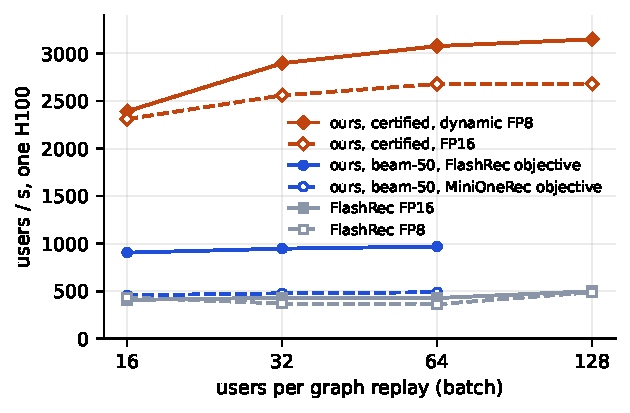
\includegraphics[width=0.92\linewidth]{flashrec_throughput.pdf}
\vspace{-3mm}
\caption{Throughput on one H100. Under FlashRec's own objective our engine's beam-50 serves about 2$\times$
FlashRec; the certified decoder with bridges serves 2.7$\times$ our beam (FlashRec and certified: one allocation;
our beam-50: the allocation of Table~M\ref{M-tab:speed}).}
\label{fig:throughput}
\vspace{-3mm}
\end{figure}

\paragraph{Against FlashRec.} On the same H100 and prompts, FlashRec takes 11.48\,ms (BF16) or 11.71\,ms (FP16)
per request and serves 408--500 users/s. Its default FP8 is slower (14.22\,ms) and costs $-0.90\,[-1.32,-0.47]$
HR@10 on this 1.5B model. In that allocation the deployed certified decoder takes 2.57\,ms (2.83\,ms with the
SASRec term) and serves 2,310--2,681 users/s (3,148 with dynamic FP8), so it is 4.5$\times$ faster per request
with 5.4--6.4$\times$ the throughput (Fig.~M\ref{M-fig:headline}). That gap splits into two factors. Our engine runs
beam-50 under FlashRec's own objective in 5.2\,ms at 970 users/s, about 2.2$\times$ FlashRec. The decoder adds
about 2$\times$ on top. The engine factor does not depend on where the timer stops: FlashRec's GPU kernels alone
take 6.78\,ms per request (1,878 kernels, profiled over 50 requests), and the rest of its 11.7\,ms is host-side
scheduling.

\paragraph{Long candidate lists.} A certified top-500 takes 2.92\,ms with bridges. Beam-500 takes 7.2\,ms under
trie scoring and 18.1\,ms under MiniOneRec's objective, and serves 253 and 71 users/s against 450. The second
forward grows with the number of multi-child prefixes the certificate needs (about $0.4K$), not with the beam
width.


\section{Detailed results on quality and fusion (main RQ2)}
\paragraph{The decoder improves quality before fusion.} On Office, certified decoding with the cbtrie objective
reaches HR@10 0.1677 at full depth and 0.1689 with bridges, against 0.1589 for MiniOneRec's FP32 beam decode of
the same checkpoint (Table~M\ref{M-tab:quality}). This gain comes from the scoring rule, not from exactness. Restricted
normalizations, which production engines adopt for speed, score better than the training objective even under
beam-50 (HR@10 0.1667 codebook, 0.1648 trie, vs.\ 0.1589 full), and the validation-tuned weight
$w_c=0.75$ discounts the third code, which carries a catalog-structure penalty unrelated to the user
(Appendix~\ref{app:objective}). On Industrial, no scoring rule significantly beats the original objective,
and certified decoding is at least as good as beam (Table~M\ref{M-tab:quality}).

\paragraph{Fusion changes what is retrieved.} Adding $\beta\log q_{\text{SASRec}}$ inside the certified search
raises Office HR@10 by $+1.36$ points. That is $+2.36$ over MiniOneRec's own decode, with no LLM training, and
on par with the best \emph{trained} result we know of on this split (0.1834~\cite{ax2608.20611}). Reranking the
LLM's top-50 with the same term recovers most of the HR@10 gain (with bridges at 18/22: 0.1800 vs.\ 0.1825 fused,
$\Delta=+0.25\,[+0.08,+0.43]$). It cannot change the candidate set, so its HR@50 does not move, while fusion adds
2.26 points. At $K=500$ fusion lifts HR@500 from 0.504 to 0.543 on
Office and from 0.523 to 0.544 on Industrial. Certification is unaffected: 100\% of Office users certify the
fused top-10. The fused top-500 needs $M=256$ on Office; on Industrial, $M=512$ (4.23\,ms) certifies all users.

\paragraph{Reranking fails when the term matters.} With a synthetic item value $\lambda v$, $v\sim\mathcal N(0,1)$,
reranking the LLM's top-50 recovers 99.2\% of the exact top-10 at $\lambda=0.5$ but only 50.0\% at $\lambda=2$.
Certified search stays exact. Filters behave the same way: when 5\% of items are eligible, filtering the LLM's
top-50 recovers only 30.5\% of the exact eligible top-10. Two certified forwards return it exactly, and
filter-after-retrieval needs a 10$\times$ longer list to catch up.

\paragraph{Against FlashRec.} Paired against FlashRec FP16, certified decoding gains $+0.45\,[+0.00,+0.90]$
HR@10 and the fused decoder gains $+1.81\,[+1.23,+2.36]$. Part of FlashRec's deficit is numerical. On our Qwen2
port, its first-code log-probabilities differ from the reference model by 0.23 nats on average. We could not
attribute this to any component we could isolate (Appendix~\ref{app:flashrec}). We therefore also compare with
our exact implementation of FlashRec's objective (HR@10 0.1679). Certified decoding matches it at half the
latency ($+0.10\,[-0.31,+0.58]$), and fusion adds $+1.46\,[+0.88,+2.01]$.


\section{Catalog scaling (main RQ3)}
\paragraph{Catalog size.} The released catalogs are small, but the model's codes address
$88\times256\times256=5.8$M SIDs. We densify the trie up to 1M SIDs, by adding siblings under real prefixes or
new prefixes under real first codes, and score real prompts with the real model (Fig.~M\ref{M-fig:catalog}). Quality
has no meaning for synthetic items, but cost does. The minimal expansion is flat in catalog size, at
$|N|\approx8.4/42/410$ for $K=10/50/500$ from 10k to 1M SIDs, and so is latency at a fixed budget: 6.33\,ms on
the real catalog and 6.36\,ms at 1M SIDs (A6000, $M=16$). Forward~1 always carries the prompt and the 88 first
codes, and Forward~2 carries $M$ rows. Certified top-10 holds for at least 99.6\% of users at $M=16$ and for 100\%
at $M=32$, at every size. Industrial replicates this ($|N|\approx7.8/38/350$). The two-sided guarantee does
\emph{not} scale: $|E|$ grows with branching as the $-\log n_p$ lower bound loosens. On dense tries, Forward~2
should therefore be sized by a fixed $M$, with a fallback for the rare uncertified request.

\paragraph{Serving at 1M SIDs.} With both bridges, the deployed decoder takes 2.65--2.89\,ms on the 1M-SID catalog
(2.60\,ms on the real one). Rerunning the 0.2\% of requests whose top-10 is not certified at $M=16$ with $M=32$
gives a p99 of 2.98\,ms, including the reruns. Fusion is the harder case. A per-item term enters each prefix's
bound through its maximum over the prefix's items. With thousands of items per prefix, that maximum is almost
always large, so the bound loosens. With a random term ($\sigma=0.5$ nats) on 1M SIDs, $M=16$ certifies only 16\%
of top-10s. $M=64$ certifies 96\%, $M=128$ certifies 100\% at 2.97\,ms, and $M=512$ certifies 100\% of top-50s at
3.19\,ms. A weaker term ($\sigma=0.1$) needs only $M=64$. These timings include the catalog-wide scatter-max and a
4\,MB host-to-device copy of the term per request. The budget must therefore scale with the term's strength and
the catalog's density; the certificate reports when it was too small.




\section{Late entry in detail (main RQ4)}
Table~M\ref{M-tab:late} shows that early exit loses 2.4--3.7 points of HR@1, since the top-1 changes for half of
the users. Late entry with a distilled bridge is statistically indistinguishable from full depth on HR@10 and
NDCG@10 on both datasets. The prefix-weighted KL loss matters: with a uniform loss, HR@1 drops by 0.35 points on
Industrial. With 2 to 14 remaining layers, the distilled bridge stays within $-0.09$ to $+0.14$ points of
full-depth HR@10 (Appendix~\ref{app:extra}). The deployed configuration enters the first code at layer 18 and the third at layer
26. Against the full-depth model its HR@10 ($+0.12\,[-0.27,+0.51]$) and NDCG@10 ($0.00\,[-0.20,+0.20]$) are
statistically unchanged, and it cuts the certified top-10 from 4.35 to 2.75\,ms on an H100. It is not a copy of
the full-depth ranking: top-1 agrees for 79.8\% of users and the top-10 sets overlap by 77\%. The bridged model is
a different ranker of equal measured quality, and the certificate is a statement about it, not about the
full-depth model. The difference lies in the objective, not the search: scored exhaustively, the bridged and
full-depth models agree on top-1 for 79.6\% of users. Nearly all of it comes from the first-level bridge. With
only the third-code bridge (layer 22), top-1 agrees for 95.8\% of users and the top-10 overlap is 94\%
(Table~M\ref{M-tab:speed}), at 3.06 instead of 2.61\,ms. That configuration is the faithful choice when agreement
with the full model matters. The first-level bridge's held-out KL was still falling when we stopped training on
4,600 validation prompts. Because distillation uses no labels, the training split's prompts can be used as well.
Distilling both bridges on 38,000 training-split prompts cuts its held-out KL by 44\% and raises agreement with
the full-depth model to 85.4\% (top-1) and 82.5\% (top-10 overlap), at the same 2.60\,ms. Quality is unchanged
(HR@10 0.1697, $+0.21\,[-0.16,+0.58]$ against full depth). Late entry of the \emph{second} code below layer
18 is a trade-off (NDCG@10 $-0.25\,[-0.51,-0.01]$). That code decides set membership, so we stop at 18. The best
entry layer depends on the model: 26 for the released Office model, 22 after one more fine-tuning epoch, and 18
on Industrial. We choose it on validation.


\section{Other backbones}
\label{sec:exp-backbones}



We test public MiniOneRec-format checkpoints that we did not train (Table~M\ref{M-tab:backbones}). Certification
and the 1.8--1.9$\times$ full-depth speedup carry over unchanged to a deeper 3B and a wider 7B model. Certified
top-10 is 99.8--100\% everywhere, and certified decoding matches beam-50 on HR@10 ($+0.12$ and $+0.04$, n.s.).
The third-code bridge, trained with the same recipe, is lossless on both ($-0.06$, $-0.02$, n.s.). It brings the
3B and 7B to 2.8$\times$ and 2.7$\times$ their own beam-50. Fusion helps more when the LLM is weaker: the same
SASRec term adds 2.2--2.4 HR@10 and lifts both above the released 1.5B LLM alone. An RL-tuned (GDPO) checkpoint
makes certification \emph{cheaper}: top-50 certifies at $M=16$ for 26--31\% of users, against 14--20\% for its SFT
parent. RL sharpens the distribution, so fewer prefixes cross the bound.



\section{OpenOneRec: numerics and the small-tokenizer contrast (main RQ5)}
\paragraph{Numerics.} In BF16 a request's scores depend slightly on the shape of the batch that computes them.
Our engine's scores agree with sequential Hugging Face decoding to within 0.10--0.24 nats, and its top-10 overlaps
the reference search's by 90--96\%. Certified lists from different budgets differ only by near-ties within
0.26 nats of the tenth score. Each certificate is exact for the scores its forward computed. Computing the
LM head's output in FP32 matters: BF16 logits of magnitude around 30 are rounded in steps of 0.125 and create
spurious ties; with BF16 logits the largest disagreement between budgets on video doubled (0.18 vs.\ 0.09
nats).

\paragraph{Contrast with a small tokenizer.} On MiniOneRec a first-level budget does not pay. All 88 first codes
fit into the fused prompt forward (2.65\,ms), while a budget adds a pass and, because its first-level prior is
flat, certifies a top-10 for only 61\% of users at $A_1=32$ and 85\% at 48. Widening its first level synthetically
from 88 to 600 codes raises the fused decoder from 2.64 to only 3.47\,ms. The two regimes call for the two forms of
the same certificate.


\section{Serving conditions on MiniOneRec}
\label{sec:exp-applied}

\begin{table}[t]
\caption{Serving conditions (MiniOneRec Office, H100, FP16, batch 1, median ms; p99 where requests that do not
certify are rerun with every prefix expanded). Long-history rows use synthetic content and measure latency only.}
\label{tab:applied}
\vspace{-2mm}
\footnotesize
\setlength{\tabcolsep}{1.5pt}
\begin{tabular*}{\linewidth}{@{\extracolsep{\fill}}lrrr@{}}
\toprule
setting & certified & beam-50 & top-10 \\
\midrule
\multicolumn{4}{@{}l}{\emph{full-vocabulary objective, no forced suffix}} \\
$M=64$ / + fallback (p99)                      & 5.22 / 28.5  & 5.82  & 94\% / 100\% \\
bridge, $M=256$ / + fallback (p99)             & 4.55 / 17.5  & --    & 99\% / 100\% \\
every prefix, full depth / bridged             & 23.2 / 13.2  & --    & 100\% \\
\multicolumn{4}{@{}l}{\emph{full vocabulary + forced suffix (MiniOneRec's objective)}} \\
$M=64$ / $M=512$                               & 7.85 / 16.3  & 8.34  & 52\% / 89\% \\
\midrule
\multicolumn{4}{@{}l}{\emph{long user histories}} \\
cached, 1k / 4k / 8k tokens                    & 3.66 / 6.54 / 10.4 & 7.19 / 13.1 / 20.7 & 100\% \\
uncached, 1.1k / 3.15k tokens                  & 7.59 / 21.4  & 11.5 / 37.0 & 100\% \\
uncached 3k, users/s ($B=16$)                  & 51           & 32    & -- \\
\bottomrule
\end{tabular*}
\vspace{-3mm}
\end{table}

\paragraph{Without trie normalization.} Normalization is a decode-time choice: the model is trained with
full-vocabulary cross-entropy either way, and on Office the restricted rules score better
(\S M\ref{M-sec:rq2}). Some deployments still serve the full-vocabulary objective, for example to keep scores
calibrated across catalogs, as OpenOneRec does. We serve it exactly (Table~\ref{tab:applied}). Without the forced
suffix, a budget of $M=64$ certifies 94\% of top-10s and costs less than beam-50 (5.22 vs.\ 5.82\,ms). The rest are
rerun with every prefix expanded, which costs 23\,ms at full depth. The median stays at 5.2\,ms, but the tail moves
to 28.5\,ms at p99. With the third-code bridge, $M=256$ certifies 99\% at 4.55\,ms, and the p99 including reruns is
17.5\,ms. The forced suffix is what makes MiniOneRec's original objective expensive. Its two extra terms are not
bounded by the prefix, so certification needs a third forward over items: $M=512$ certifies 89\% at 16.3\,ms, twice
beam's cost. The dependence on normalization is therefore one of degree. Trie-style rules certify every request at
a flat cost, the full-vocabulary objective is served exactly at beam's median cost with a heavier tail, and the
forced suffix roughly doubles it.

\paragraph{Long user histories.} Production systems keep a user's history K/V across requests and process only
the new tokens. We emulate that with a long history held in the prompt cache. At 1k, 4k and 8k cached tokens the
deployed decoder takes 3.66, 6.54 and 10.4\,ms against 7.19, 13.1 and 20.7\,ms for beam-50, a constant
2.0$\times$. Every new row attends over the whole history, and beam has 50 such rows in 28 layers, while certified
decoding has 16 in two. Without a cache the prompt forward dominates. Per request the gain stays 1.5--1.7$\times$
(7.59 vs.\ 11.5\,ms at 1.1k tokens; 21.4 vs.\ 37.0\,ms at 3.15k), but throughput becomes prefill-bound and the gain
shrinks from 2.7$\times$ to 1.6$\times$ (51 vs.\ 32 users/s at 3k tokens). Long contexts therefore dilute the
speedup only when histories are not cached. These runs use streaming (online-softmax) versions of our Triton
attention kernels for prompts over 256 tokens.


\section{Engine and latency ladder}
\label{app:engine}

\begin{table}[h]
\caption{Latency ladder, Office, batch 1, median ms. The A6000 rows come from one allocation, as do the H100
rows; the final rows are from a later allocation.}
\label{tab:ladder}
\vspace{-2mm}
\small
\setlength{\tabcolsep}{3pt}
\begin{tabular*}{\linewidth}{@{\extracolsep{\fill}}lrr@{}}
\toprule
step & A6000 & H100 \\
\midrule
Hugging Face \texttt{generate}, FP32                 & 868.8 & -- \\
our engine, FP32, beam-50                            & 100.8 & 48.3 \\
BF16, one CUDA graph per request                     & 42.1  & 20.1 \\
+ \texttt{torch.compile}                             & 35.0  & 12.9 \\
+ first trie level fused into the prompt forward     & 28.1  & 8.50 \\
+ FP16, cached prompt template                       & 26.2  & 8.48 \\
certified exact decoding (trie)                      & 14.4  & 5.57 \\
+ multi-child prefixes only, Triton prompt attention & 13.25 & 4.37 \\
+ late entry, third code at layer 22                 & 8.98  & 3.32 \\
+ first level at 18, third code at 26 (final)        & 6.38  & 2.75 \\
+ SASRec term (in the graph on the H100)             & 6.44  & 2.89 \\
\bottomrule
\end{tabular*}
\end{table}

FP16 with a pre-scaled query matches FP32's top-1 for 500/500 cohort users; BF16 matches for 488/500. On the H100
the engine is bound by kernel count, not bandwidth. The first certified decoder issued 2,555 kernels and spent
5.9\,ms of GPU time per request. Late entry and a Triton prompt attention cut this to 1,474 kernels and 3.7\,ms.
Fusing the forced suffix into one two-token forward saves 10\,ms on the A6000 for the beam baselines.

\section{What exact decoding reveals about the objective}
\label{app:objective}

\begin{table}[h]
\caption{Scoring rules under beam-50, Office, all test users.}
\label{tab:scoring}
\vspace{-2mm}
\footnotesize
\setlength{\tabcolsep}{3pt}
\begin{tabular*}{\linewidth}{@{\extracolsep{\fill}}lrrrr@{}}
\toprule
scoring rule & HR@1 & HR@10 & NDCG@10 & HR@50 \\
\midrule
full vocabulary + suffix (MiniOneRec) & 0.0947 & 0.1589 & 0.1249 & 0.2370 \\
full vocabulary, no suffix            & 0.0986 & 0.1624 & 0.1284 & 0.2363 \\
trie                                  & 0.0982 & 0.1648 & 0.1287 & 0.2417 \\
codebook (FlashRec)                   & 0.0986 & 0.1667 & 0.1299 & 0.2470 \\
\bottomrule
\end{tabular*}
\end{table}

\paragraph{Beam search error grows with list length.} From exhaustive FP32 scores of every SID for every user,
beam-$W$ under the full objective recovers 49\%, 53\% and 64\% of the exact top-$W$ for $W=50$, 100 and 500
(Industrial: 67/69/79\%). Under trie scoring it recovers 95/96/99.6\%. Under the full objective, exact search
\emph{loses} recall at large $K$ (HR@500 $-4.3\,[-5.3,-3.2]$ vs.\ beam-500). Under the validation-tuned codebook
objective it \emph{gains} recall (HR@500 $+2.4\,[+1.4,+3.3]$). Beam search's prefix-first pruning acts as an
implicit depth discount; once the discount is explicit, exactness stops hurting.

\paragraph{Why the deep terms mislead.} Over 1,217 Office users $\times$ 3,444 SIDs:
(i) \emph{Sibling penalty}: $\lp(c\mid a,b)$ falls with the number of catalog items sharing $(a,b)$, with median
$-0.87$, $-2.46$, $-3.05$, $-3.38$ and $-4.12$ for 1, 2, 3, 4 and 6 siblings. That is steeper than an even split,
a structural penalty unrelated to the user (Fig.~\ref{fig:sibling}).
(ii) \emph{Codebook leakage}: even after a valid $(a,b)$, a median 47\% of next-token mass falls outside the
$c$-codebook, which full normalization charges unevenly.
(iii) The forced suffix acts as a weak popularity prior ($r=0.15$ with log popularity). It moves the target up
for 28\% of users and down for 25\%.

\begin{figure}[h]
\centering
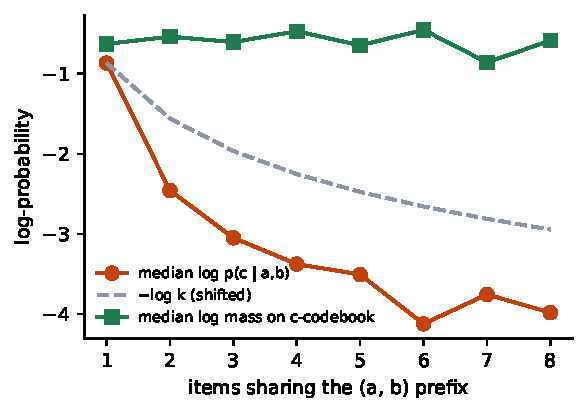
\includegraphics[width=0.8\linewidth]{sibling_penalty_office.pdf}
\vspace{-3mm}
\caption{The sibling penalty (Office, exhaustive FP32 scores).}
\label{fig:sibling}
\end{figure}

\section{FlashRec comparison details}
\label{app:flashrec}
We use FlashRec 0.1.2 (commit 1089682, Apache-2.0). Our patch adds Qwen2's QKV bias and removes QK-norm. When
there is no norm, it runs FlashRec's fused RoPE + FP8 K/V-store Triton kernel with the normalization disabled.
FlashRec's CUDA graphs are captured at 19 sizes, and its JIT trie kernel is verified loaded. Latency is the wall
time of \texttt{engine.generate()} from token ids to ranked beams on the host. Ours is a pinned host prompt through
one graph replay; copying the list back to the host adds 0.02\,ms.

\begin{sloppypar}
\emph{Numerical drift.} On our port, FlashRec's first-code log-probabilities differ from Hugging Face FP32 by 0.23
nats on average. Hugging Face in half precision differs by 0.002 (FP16) and 0.02 (BF16). FlashRec's top-1 agrees
with exact beam under the same objective for 80\% of users. The drift persists when we disable each component we
could isolate: the radix cache, CUDA graphs, fused expansion, the per-codebook head, GQA grouping (a
12-KV-head copy drifts the same), output-layer tying, Q/K layout, and its pre-cut of $2\times$ the beam width in
candidates.
We report FlashRec as measured and also our exact implementation of its objective. Speed is unaffected, since
the computation is the same.
\end{sloppypar}

\section{Additional results and negative results}
\label{app:extra}
\emph{Late-entry depth.} With a uniform-KL bridge on Office, keeping 2/4/10/14 layers gives HR@10 deltas of
$-0.09/+0.04/\text{n/a}/+0.14$ and HR@1 deltas of $-0.45/-0.27/+0.06/-0.02$; top-1 agrees with full depth for 86--94\% of
users.
\emph{One forward is not enough.} A user-independent table of third-code scores keeps HR@10 within 0.9 points
but halves HR@1 (0.098 $\to$ 0.050). Guessing the expansion set before Forward~1, from history or popularity,
covers the certificate set for top-10 in at most 29\% of requests.
\emph{Quantization.} Weight-only INT8 is quality-neutral but only 3--8\% faster, and INT4 is no faster. At
50--216 rows per forward, GEMMs are past the regime where weight-only kernels help. Static FP8 is slower than
BF16 on an L40S. Dynamic per-token FP8 on the H100 is quality-neutral and adds 16--21\% throughput.
\emph{Training for the decoder.} One more SFT epoch with a loss aligned to the decoder's restricted normalization
improves HR@10 by $+0.90\,[+0.27,+1.54]$ over the release. A full-vocabulary control gets almost all of it
(aligned vs.\ control $+0.14\,[-0.16,+0.47]$), so the alignment itself does not help.

\section{Reproducibility}
\label{app:repro}
\begin{sloppypar}
Code, the FlashRec patch and every run are in the repository (anonymized for review). Bridges train on the
validation split only; weights and $\beta$ are chosen on validation and evaluated once on test. Hardware: NVIDIA
H100 80GB and RTX A6000 (L40S and A40 for FP8 and catalog-scaling runs). Main runs: \texttt{runs/frLat},
\texttt{frTp} (Table~M\ref{M-tab:speed}); \texttt{finalH}, \texttt{collabO}, \texttt{fuseI} (Table~M\ref{M-tab:quality});
\texttt{lbndA} (Table~M\ref{M-tab:bounds}); \texttt{scaleP}, \texttt{scaleI} (Fig.~M\ref{M-fig:catalog});
\texttt{ladder2}, \texttt{h100M} (Table~\ref{tab:ladder}); \texttt{oo\_video}, \texttt{oo\_videoF},
\texttt{oo\_ad}, \texttt{oo\_product} (node counts, recall and hit rates in Table~M\ref{M-tab:openonerec};
\texttt{scripts/openonerec\_cert.py}, \texttt{openonerec\_analysis.py}); \texttt{oo\_latV2}, \texttt{oo\_latA2}
(latency in Table~M\ref{M-tab:openonerec}; \texttt{scripts/openonerec\_latency.py},
\texttt{openonerec\_latency\_analysis.py}, both launched by \texttt{openonerec\_job.sh}).
\end{sloppypar}


\bibliographystyle{ACM-Reference-Format}
\bibliography{refs}
\end{document}
